\documentclass{IEEEtran}
\usepackage[utf8]{inputenc}

\usepackage{graphicx}
\usepackage{hyperref}
\usepackage{xurl}
\usepackage{float}
\usepackage{tabularx}

\graphicspath{{./images/}}


% correct bad hyphenation here
\hyphenation{op-tical net-works semi-conduc-tor}


\title{Propuesta de arquitectura de control de versiones en bases de datos evolutivas.}

\author{\IEEEauthorblockN{ Gerardo Adolfo Salas Montoya, Miguel Perez Montero}
\IEEEauthorblockA{\\Maestría en ingeniería de software con énfasis en arquitectura y diseño de software.\\
Universidad Cenfotec\\
San Jose, Costa Rica\\
Email: \{gsalasm, mperez\}@ucenfotec.ac.cr }}


\date{\today}



\begin{document}

\maketitle

\renewcommand{\refname}{Resumen}
\begin{abstract}
    Este artículo se centra en el estudio y la mejora de los procesos de control de versiones para bases de datos evolutivas, un área que ha recibido relativamente poca atención en la disciplina de ingeniería de software, sin embargo, es una práctica cada vez más demandada en los grupos de desarrollo. Las bases de datos están diseñadas para adaptarse y cambiar con el tiempo sin embargo el no tener un registro completo de los cambios que se aplican sobre cada uno de los objetos que la componen pueden llegar a causar diferentes problemas en los grupos de desarrollo y por su puesto en las bases de datos.
\end{abstract}

\renewcommand{\refname}{Palabras clave}
\begin{IEEEkeywords}
    Control de versiones de bases de datos,
    Bases de datos evolutivas,
    Integración/Despliegue continuo (CI/CD),
    Gestión de cambios en bases de datos,
    Arquitectura de bases de datos,
    Liquibase,
    Flyway,
    Desarrollo ágil de software
\end{IEEEkeywords}

\section{Introducción}
En el desarrollo de software moderno, las bases de datos desempeñan un rol fundamental para asegurar la adaptabilidad y flexibilidad de las aplicaciones. El concepto de bases de datos evolutivas surge como respuesta a la necesidad de las organizaciones de adaptarse rápidamente a cambios en los requisitos y necesidades del negocio, integrándose efectivamente en los procesos de Integración Continua y Despliegue Continuo (CI/CD). Sin embargo, la gestión de versiones en este tipo de bases de datos plantea desafíos significativos, ya que las herramientas tradicionales de control de versiones no están diseñadas para manejar la complejidad y estructura de las bases de datos, lo cual con frecuencia resulta en inconsistencias y problemas de implementación.

Este proyecto aborda la problemática de la falta de una arquitectura robusta de control de versiones para bases de datos evolutivas, lo cual afecta la calidad y eficiencia de los procesos de CI/CD en las organizaciones. La propuesta tiene como objetivo desarrollar una arquitectura de control de versiones específica para bases de datos que evolucionan constantemente, buscando reducir riesgos de errores y conflictos en los cambios, mejorar la consistencia de los datos y facilitar la integración rápida y frecuente de nuevas características. Además, esta solución permitirá mantener un registro exhaustivo de todos los cambios, apoyando tanto la implementación de mejoras como la corrección de errores.

Desde el punto de vista técnico, herramientas como \\Liquibase y Flyway ofrecen funcionalidades clave que pueden adaptarse y optimizarse para satisfacer las necesidades de control de versiones en bases de datos. Operativamente, el proyecto es viable, ya que muchas organizaciones ya emplean prácticas de control de versiones en sus procesos de CI/CD, y la integración de una arquitectura específica para bases de datos no requerirá cambios disruptivos, sino mejoras y adaptaciones efectivas.

Conforme al paradigma Objetivo-Pregunta-Métrica (GQM) \cite{Basili1992}, el objetivo de esta investigación se puede enunciar de la siguiente manera:

\begin{itemize}
    \item[] {\textbf{\textit{Aplicar:}}} Una arquitectura para el control de versiones en bases de datos que cambian con frecuencia.
    \item[] {\textbf{\textit{Con el propósito de:}}} mejorar la trazabilidad, consistencia y facilidad de integración de los cambios en la base de datos en entornos de CI/CD.
    \item[] {\textbf{\textit{Con respecto a:}}} los desafíos en el rastreo y gestión de cambios en bases de datos.
    \item[] {\textbf{\textit{Desde el punto de vista de:}}} investigadores y profesionales de ingeniería de software enfocados en control de versiones y prácticas de integración y despliegue continuo.
    \item[] {\textbf{\textit{En el contexto de:}}} mejorar las prácticas de control de versiones en organizaciones que dependen de actualizaciones frecuentes de bases de datos como parte de sus flujos de trabajo.
\end{itemize}


\vspace{0.5cm}
La estructura del resto del artículo es la siguiente. La Sección II presenta las preguntas de investigación. La sección III discute los trabajos relacionados y el estado del arte. Los antecedentes se describen en la sección IV. La metodología de investigación se explica en la sección V, y los objetivos se presentan en las secciones VI y VII. La sección VIII muestra los resultamos obetenidos por medio de las encuentas y las entrevistas a profesionales. La Sección IX aborda la descripción de la arquitectura propuesta para el control de cambios en bases de datos y su implementación utilizando herramientas como liquibase y flyway y por ultimo la sección X describe las pautas de la solucion en conclusiones y presentan el posible trabajo futuro.


\section{Preguntas de Investigación.}
Esta sección enumera las principales preguntas de investigación que se pretende responder:
\begin{itemize}
    \item ¿Cómo mantener la integridad del esquema de base de datos a lo largo del tiempo? 
    \item ¿Cómo colaborar efectivamente entre equipos de desarrollo y administradores de bases de datos? 
    \item ¿Cuál es el impacto de la implementación de un sistema de control de versiones en la integridad y consistencia de los datos?
\end{itemize}


\section{Trabajos Relacionados}
La siguiente investigación se ha realizado con un enfoque en el control de versiones dentro del contexto de la arquitectura de bases de datos:

En el 2006, Ambler y Sadalage \cite{ambler2006refactoring} presentan en su obra una guía exhaustiva sobre la refactorización de bases de datos en entornos de desarrollo ágil. El libro se enfoca en cómo aplicar técnicas de refactorización para mejorar el diseño, la mantenibilidad, la extensibilidad y el rendimiento de las bases de datos. Los autores explican cómo realizar pequeños cambios en las estructuras de tablas, datos, procedimientos almacenados y disparadores sin modificar la semántica de la base de datos. Además, se detalla el proceso de evolucionar los esquemas de bases de datos al mismo ritmo que el código fuente en proyectos ágiles. La obra proporciona ejemplos prácticos y casos aplicados con Oracle y Java, adaptables a otras plataformas como CSharp, C++ y SQL Server. Su principal objetivo es ofrecer estrategias para reducir el desperdicio, el retrabajo, los riesgos y los costos en el desarrollo de bases de datos, haciendo posible su evolución en entornos productivos complejos.

Luego en el 2007, Sadalage \cite{sadalage2007recipes} aborda la integración continua de bases de datos dentro de equipos ágiles, un desafío común debido a la dificultad de integrar continuamente la base de datos con el código de la aplicación. El autor defiende que el Desarrollo Evolutivo de Bases de Datos puede ser perfectamente compatible con los métodos ágiles, como el Desarrollo Guiado por Pruebas (TDD) y la Programación en Pareja. Este enfoque facilita a los equipos de desarrollo realizar modificaciones constantes en la base de datos sin comprometer la eficacia de las prácticas ágiles. A través de este trabajo, Sadalage demuestra que la integración continua de bases de datos no solo es posible, sino beneficiosa para mantener la calidad y confiabilidad del software a lo largo de todo el ciclo de desarrollo.


Spinellis \cite{spinellis2005version} discute en su artículo la importancia de los sistemas de control de versiones (VCS) en el desarrollo de software. El autor subraya que, aunque muchos programadores no escribirían código de producción sin la ayuda de un editor o un compilador, muchos proyectos de software no utilizan un VCS, lo cual puede ser perjudicial a largo plazo. Spinellis argumenta que la adopción de un VCS puede mejorar la eficiencia y reducir el riesgo de errores en los proyectos, aunque su implementación requiere un esfuerzo inicial que muchas veces es percibido como un obstáculo. A través de este artículo, se destaca cómo un buen sistema de control de versiones puede ser una de las mejoras más significativas para los equipos de desarrollo.


Fluri, Fornari y Pustulka \cite{fluri2023measuring} abordan los beneficios de integrar prácticas de CI/CD (Integración Continua / Entrega Continua) en el desarrollo de aplicaciones de bases de datos. A través de estudios de caso industriales, los autores demuestran que la automatización de la integración y el despliegue de bases de datos mediante CI/CD reduce los fallos de despliegue, mejora la estabilidad del sistema y aumenta la frecuencia de los despliegues. Además, desde una perspectiva cualitativa, los desarrolladores informan una carga cognitiva reducida y mejoras en la calidad del software. Los resultados cuestionan las prácticas actuales de lanzamiento de bases de datos, que a menudo están impulsadas por expectativas comerciales y ventanas de lanzamiento fijas.


Por otra parte, Cao \cite{cao2022estimating} presenta un estudio empírico sobre la estimación del esfuerzo en el desarrollo ágil de software, evaluando diversas actividades como el desarrollo de características, la corrección de errores y la refactorización. Los resultados del estudio indican que, en contraste con la creencia popular, la precisión de las estimaciones de esfuerzo no mejora con el tiempo en el desarrollo ágil. Este estudio revela que las tareas de corrección de errores y refactorización tienden a ser sobreestimadas, mientras que las tareas de desarrollo de características no muestran tal patrón. Esta investigación aporta nueva información sobre las dificultades de estimación en el contexto de metodologías ágiles, la cual es de relevancia con el proposito de este proyecto.


Roddick \cite{roddick1992schema} explora en su artículo la evolución de esquemas en los sistemas de bases de datos, un tema crucial para garantizar que los sistemas se adapten a los cambios del mundo real mediante modificaciones en la estructura del esquema. Por lo que destaca la importancia de retener estados anteriores del esquema para asegurar la confiabilidad y la integridad de los datos. El autor aborda los desafíos que enfrentan los administradores de bases de datos al tomar decisiones sobre la validez de los datos existentes cuando se implementa un nuevo esquema. La evolución de esquemas se presenta como una propiedad esencial para la adaptación y la gestión de los sistemas de bases de datos a lo largo del tiempo.

Las fuentes de información que se mencionan, como IEEE, ACM, Research Gate entre otras, proporcionan una base sólida para entender las prácticas actuales en el desarrollo de software y la gestión de bases de datos. Los trabajos revisados destacan la importancia del uso de sistemas de control de versiones, como se observa en el estudio de Spinellis \cite{spinellis2005version}, que subraya cómo estos sistemas mejoran la productividad y reducen los riesgos asociados al desarrollo de software. Por otro lado, el trabajo de Fluri et al. \cite{fluri2023measuring} aborda la integración continua y entrega continua (CI/CD) en el contexto de bases de datos, demostrando cómo la automatización de estos procesos puede mejorar la estabilidad y eficiencia en los proyectos de desarrollo. Además, la evolución de esquemas en sistemas de bases de datos, un tema tratado por Roddick \cite{roddick1992schema}, es fundamental para asegurar que las bases de datos puedan adaptarse a los cambios sin comprometer la integridad de los datos. Finalmente, la investigación de Cao \cite{cao2022estimating} sobre la estimación de esfuerzos en el desarrollo ágil ofrece perspectivas valiosas sobre cómo las metodologías ágiles impactan en la precisión de las estimaciones de trabajo, un aspecto crítico en proyectos complejos. Estos trabajos no solo enriquecen la comprensión de los procesos ágiles y su integración con la gestión de bases de datos, sino que también forman la base para las soluciones propuestas en esta investigación.


\section{Antecedentes}

Dada la investigación realizada se aprecia como muchos autores consideran que el campo de las bases de datos ha experimentado una evolución significativa, impulsada por la necesidad de adaptarse a los cambios rápidos del entorno de desarrollo ágil y las metodologías de integración continua (CI) y entrega continua (CD). La gestión de versiones y la refactorización de bases de datos, temas clave en este estudio, han sido objeto de múltiples investigaciones. Uno de los trabajos más relevantes en este campo es el de Ambler y Sadalage (2006) \cite{ambler2006refactoring}, quienes introdujeron las técnicas de refactorización de bases de datos como un medio para mejorar la estructura y la calidad de los sistemas de bases de datos sin comprometer su semántica. Este enfoque permite que las bases de datos evolucionen de manera paralela al código fuente, lo que facilita la adaptación continua en proyectos ágiles. 

En paralelo, la investigación sobre la integración de bases de datos en entornos CI/CD ha ganado relevancia, como lo demuestra el trabajo de Fluri et al. (2023) \cite{fluri2023measuring}, que mostró cómo la automatización de la integración y despliegue de bases de datos contribuye a la estabilidad y eficiencia de los proyectos de software. Sin embargo, a pesar de estos avances, sigue siendo un desafío integrar las bases de datos en los ciclos ágiles de manera eficiente y con control adecuado de versiones. Así, la evolución de esquemas en sistemas de bases de datos, descrita por Roddick (1992) \cite{roddick1992schema}, sigue siendo una cuestión crucial, ya que permite que las bases de datos se adapten a los cambios del mundo real mientras mantienen la integridad de los datos. Estos antecedentes destacan la importancia de crear una arquitectura sólida de control de versiones para bases de datos.

\section{Metodología de Investigación}
La metodología de investigación de esta propuesta adopta un enfoque mixto, integrando tanto técnicas cualitativas como cuantitativas. Según Monje (2011) \cite{Monje2011}, el enfoque mixto permite abordar de manera integral los fenómenos bajo estudio, ofreciendo una comprensión más profunda al combinar la recolección de datos descriptivos y numéricos. Este enfoque se utilizará para explorar las percepciones y prácticas relacionadas con el control de versiones en bases de datos evolutivas, utilizando técnicas como entrevistas semiestructuradas y análisis documental en el caso cualitativo, y encuestas y experimentos controlados en el caso cuantitativo.

La metodología cualitativa permite obtener una comprensión profunda de las experiencias y desafíos de los desarrolladores y administradores de bases de datos en relación con el control de versiones. Para ello, se llevaron a cabo entrevistas semiestructuradas con expertos en el área de desarrollo de software y administración de bases de datos, así como un análisis documental de los registros de cambios y manuales de proyectos reales basado en la adapcion de la ciencia de diseño \cite{RoblesVasquezNaranjo}. La selección de los participantes se realiza mediante un muestreo intencional, y los datos obtenidos se analizan a través de un enfoque de análisis temático, permitiendo identificar patrones recurrentes en las prácticas de control de versiones.

Por otro lado, el enfoque cuantitativo se aplica para medir y analizar los datos numéricos relacionados con la implementación y el rendimiento de las prácticas de control de versiones en bases de datos. A través de encuestas estructuradas, se recolectaron datos sobre la frecuencia, efectividad y desafíos de las prácticas de control de versiones, mientras que las entrevistas permiten conocer el pensamineto de expertos en el area sobre la implementación de herramientas como Liquibase y Flyway. Los datos recolectados se analizan utilizando técnicas estadísticas descriptivas e inferenciales, permitiendo obtener conclusiones más objetivas y generalizables sobre las mejores prácticas en este campo.

La integración de ambos enfoques cualitativos y cuantitativos permite obtener una visión holística del fenómeno investigado. La triangulación de los datos cualitativos y cuantitativos se llevo a cabo mediante la comparación de los resultados de las entrevistas y las encuestas, lo que permite identificar convergencias y divergencias en los hallazgos. Además, se realizaron análisis comparativos entre los resultados obtenidos mediante ambos métodos para validar y complementar los hallazgos, ofreciendo así una comprensión más robusta y completa del problema de investigación.

El uso del enfoque mixto se justifica por la complejidad del tema investigado. Esta metodología permite abordar tanto los aspectos técnicos como los humanos del control de versiones en bases de datos evolutivas, lo que proporciona una base sólida de datos empíricos. Estos datos no solo permitirán obtener conclusiones sobre el estado actual de las prácticas en este campo, sino también ofrecer recomendaciones prácticas basadas en evidencia para mejorar las prácticas de control de versiones en la gestión de bases de datos.
    
\section{Objetivo}
El objetivo general de este proyecto es proponer una arquitectura de control de versiones para bases de datos relacionales evolutivas que facilite la gestión de cambios, mejore la eficiencia y la seguridad de los procesos de CI/CD. La elección de la taxonomía de Bloom \cite{TBloom} se debe a su amplia documentación y aplicabilidad, ya que su estructuración jerárquica permite definir los objetivos de manera clara y ordenada, desde los más generales hasta los más específicos. Esto facilita una alineación adecuada con los principios del control de versiones en bases de datos dentro de entornos ágiles de desarrollo.

\section{Objetivos Específicos}
\begin{enumerate}
    \item Analizar las herramientas actuales de control de versiones para bases de datos relacionales, tales como Liquibase y Flyway, con el fin de comprender sus características, ventajas y limitaciones en entornos de CI/CD.
    \item Evaluar el impacto técnico de implementar cambios en bases de datos sin un control de versiones adecuado, con énfasis en los efectos sobre la integridad, escalabilidad y confiabilidad de las bases de datos en entornos de desarrollo ágiles.
    \item Desarrollar una arquitectura que aborde los desafíos específicos de las bases de datos evolutivas, adaptando y mejorando las prácticas actuales de control de versiones para permitir un manejo efectivo de los cambios.
    \item Probar la efectividad de la arquitectura propuesta en entornos reales de desarrollo de software, asegurando que los beneficios descritos se materialicen en la práctica y mejoren la productividad y seguridad de los procesos de desarrollo.
\end{enumerate}

\section{Resultados}
Como parte del análisis de la documentación y los datos recopilados en las encuestas y entrevistas, se obtuvieron los siguientes resultados. Las encuestas fueron aplicadas a 23 profesionales en informática, abarcando áreas como ciencia de datos, desarrollo de software e inteligencia de negocios (BI), siendo los desarrolladores de software el grupo más numeroso (39\%), como se muestra en la Figura \ref{fig:profesionalsDistribution}. Los temas de la encuesta incluyeron experiencia en bases de datos, control de versiones, metodologías ágiles y prácticas de CI/CD.

\begin{figure}[H]
    \centering
    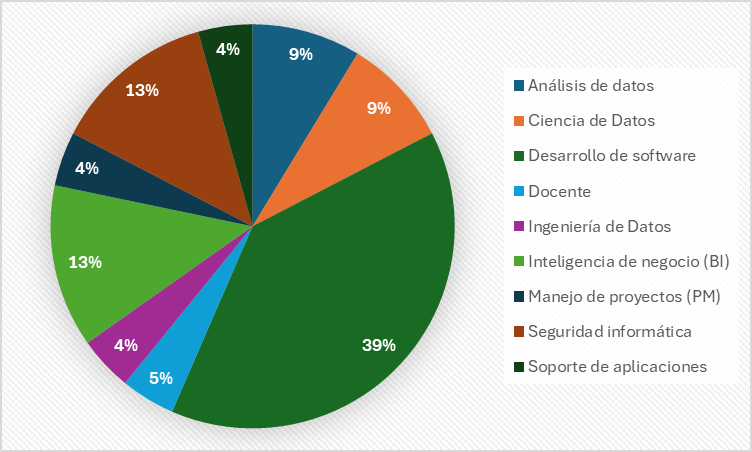
\includegraphics[width=0.45\textwidth]{images/profesionalsDistribution.png}
    \caption{Distribución de profesionales encuestados}
    \label{fig:profesionalsDistribution}
\end{figure}

En cuanto a la experiencia con bases de datos, los encuestados reportaron niveles intermedio o avanzado, donde la mayoría indica que tiene experiencia con bases de datos relacionales, pero solo un 52\% tiene experiencia con bases NoSQL. Los usuarios reportaron que los problemas más comunes al gestionar cambios en bases de datos incluyen la gestión de dependencias, conflictos de versiones y la consistencia de los datos como se puede observar en la Figura \ref{fig:commonDBIssues}.

\begin{figure}[H]
    \centering
    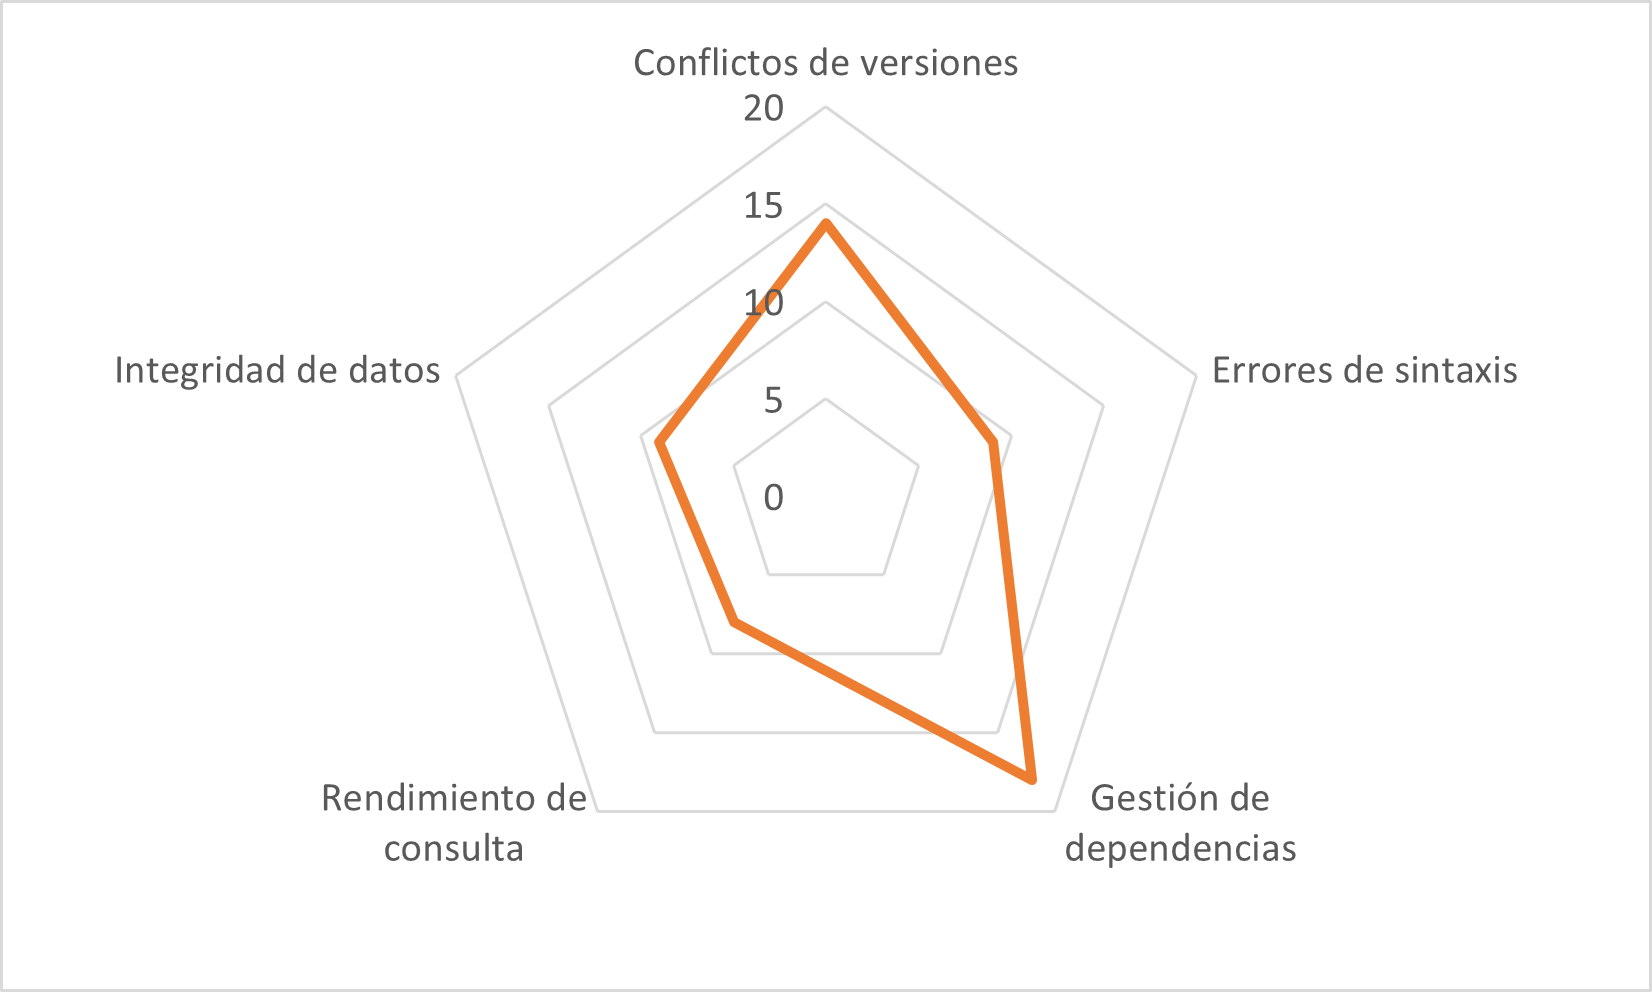
\includegraphics[width=0.45\textwidth]{images/commonDBIssues.png}
    \caption{Distribución de problemas comunes al gestionar cambios en bases de datos}
    \label{fig:commonDBIssues}
\end{figure}

Respecto al uso de sistemas de control de versiones, aunque la mayoría de los encuestados tienen experiencia (principalmente con Git), un 60\% indicó no haber usado control de versiones en bases de datos anteriormente en sus proyectos. Para facilitar la compresión de la utilización de control de versiones en bases de datos, muestran los resultados divididos por profesión, como se puede ver en el gráfico de la Figura \ref{fig:vcsDBbyProfesion}, solo una minoría de los encuestados ha aplicado sistemas de control de versiones específicamente en bases de datos.

\begin{figure}[H]
    \centering
    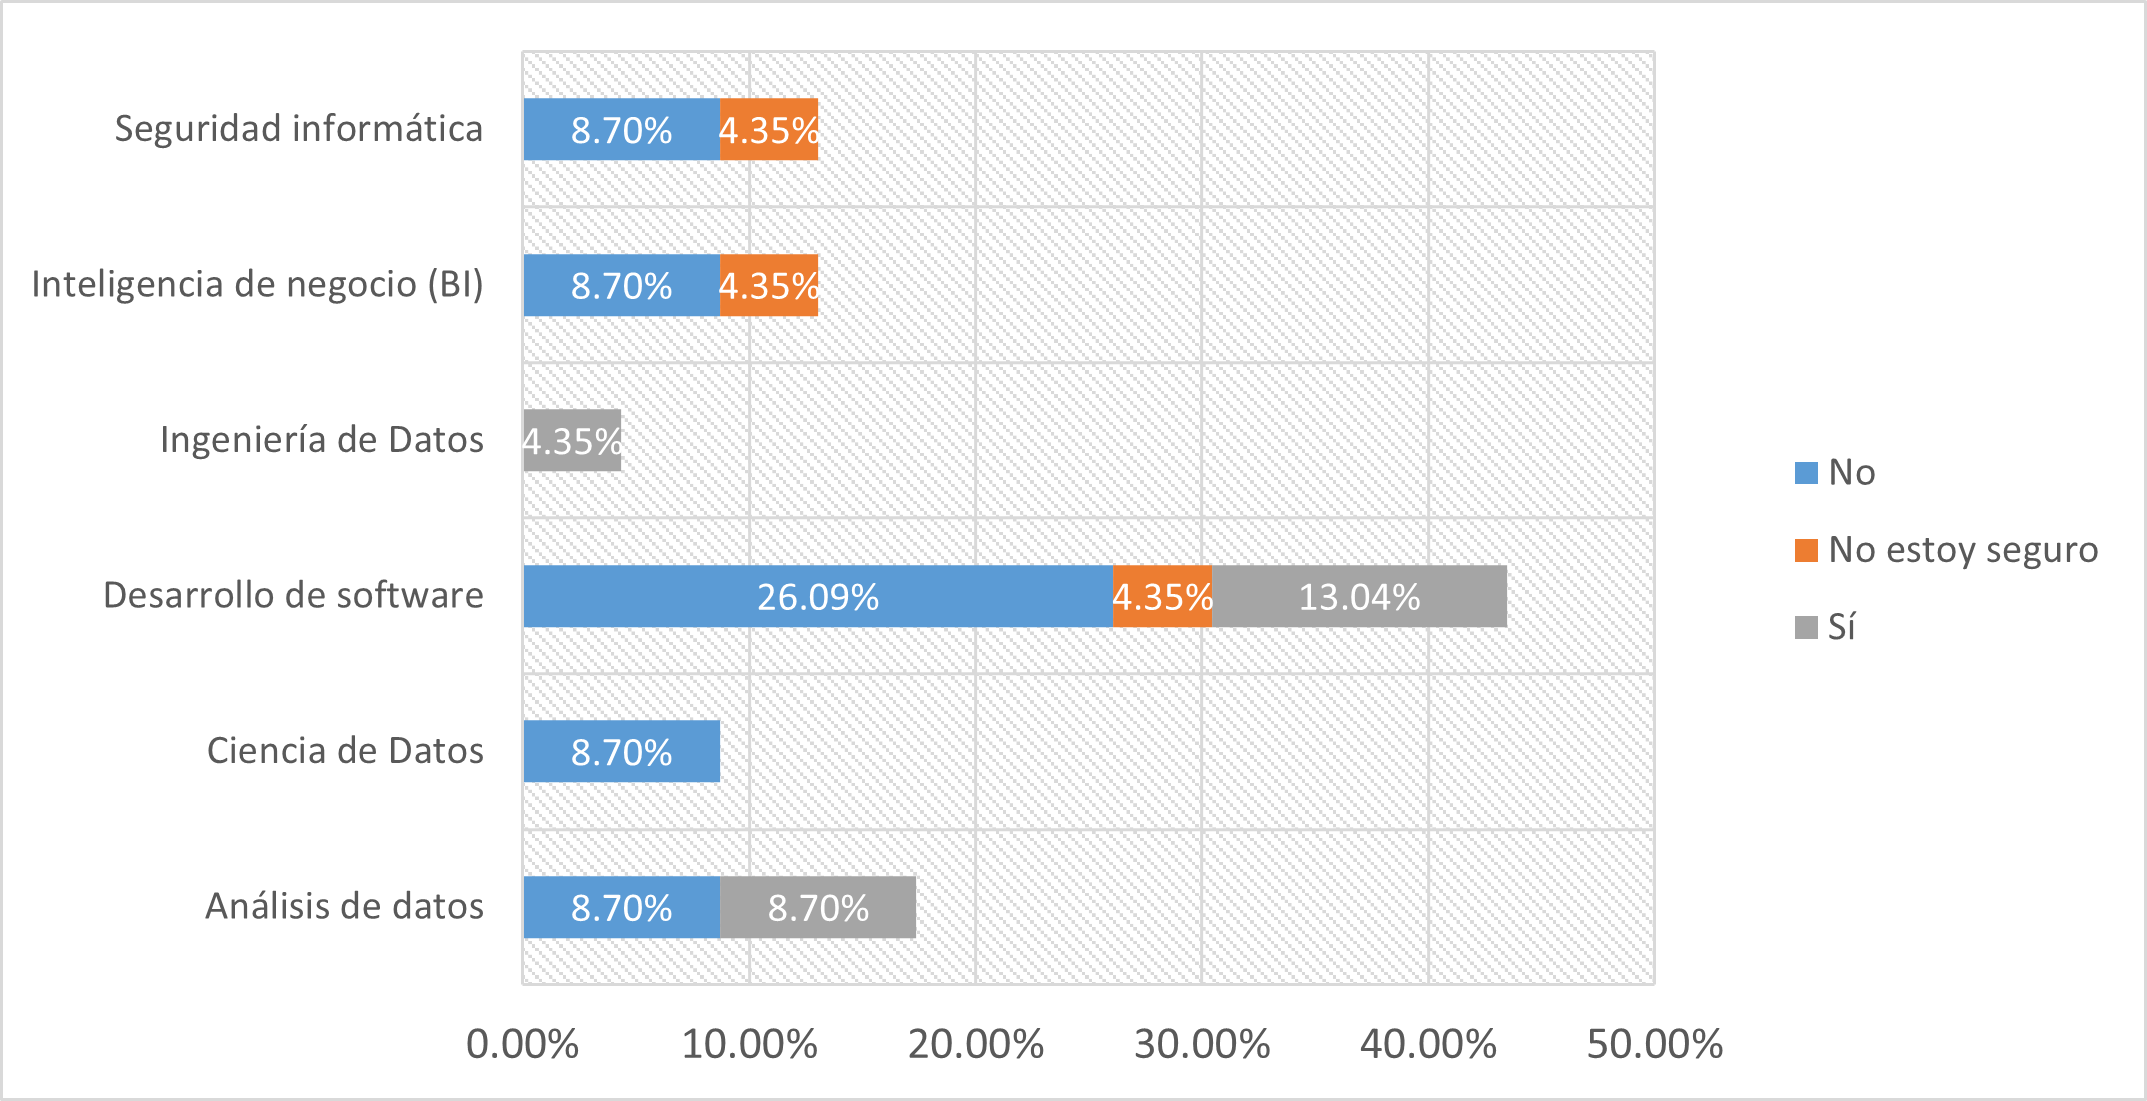
\includegraphics[width=0.45\textwidth]{images/vcsDBbyProfesion.png}
    \caption{Utilización de control de versiones en bases de datos por profesión}
    \label{fig:vcsDBbyProfesion}
\end{figure}

En términos de metodologías ágiles, más del 90\% de los encuestados indicó tener experiencia en su uso, con herramientas de planificación como Jira y Azure DevOps siendo las más utilizadas. Entre las dificultades en la estimación de tareas para bases de datos se mencionaron dependencias ocultas y cambios imprevistos, destacando la complejidad en la planificación de tareas en este contexto, como se observa en la Figura \ref{fig:dificultades}

\begin{figure}[H]
    \centering
    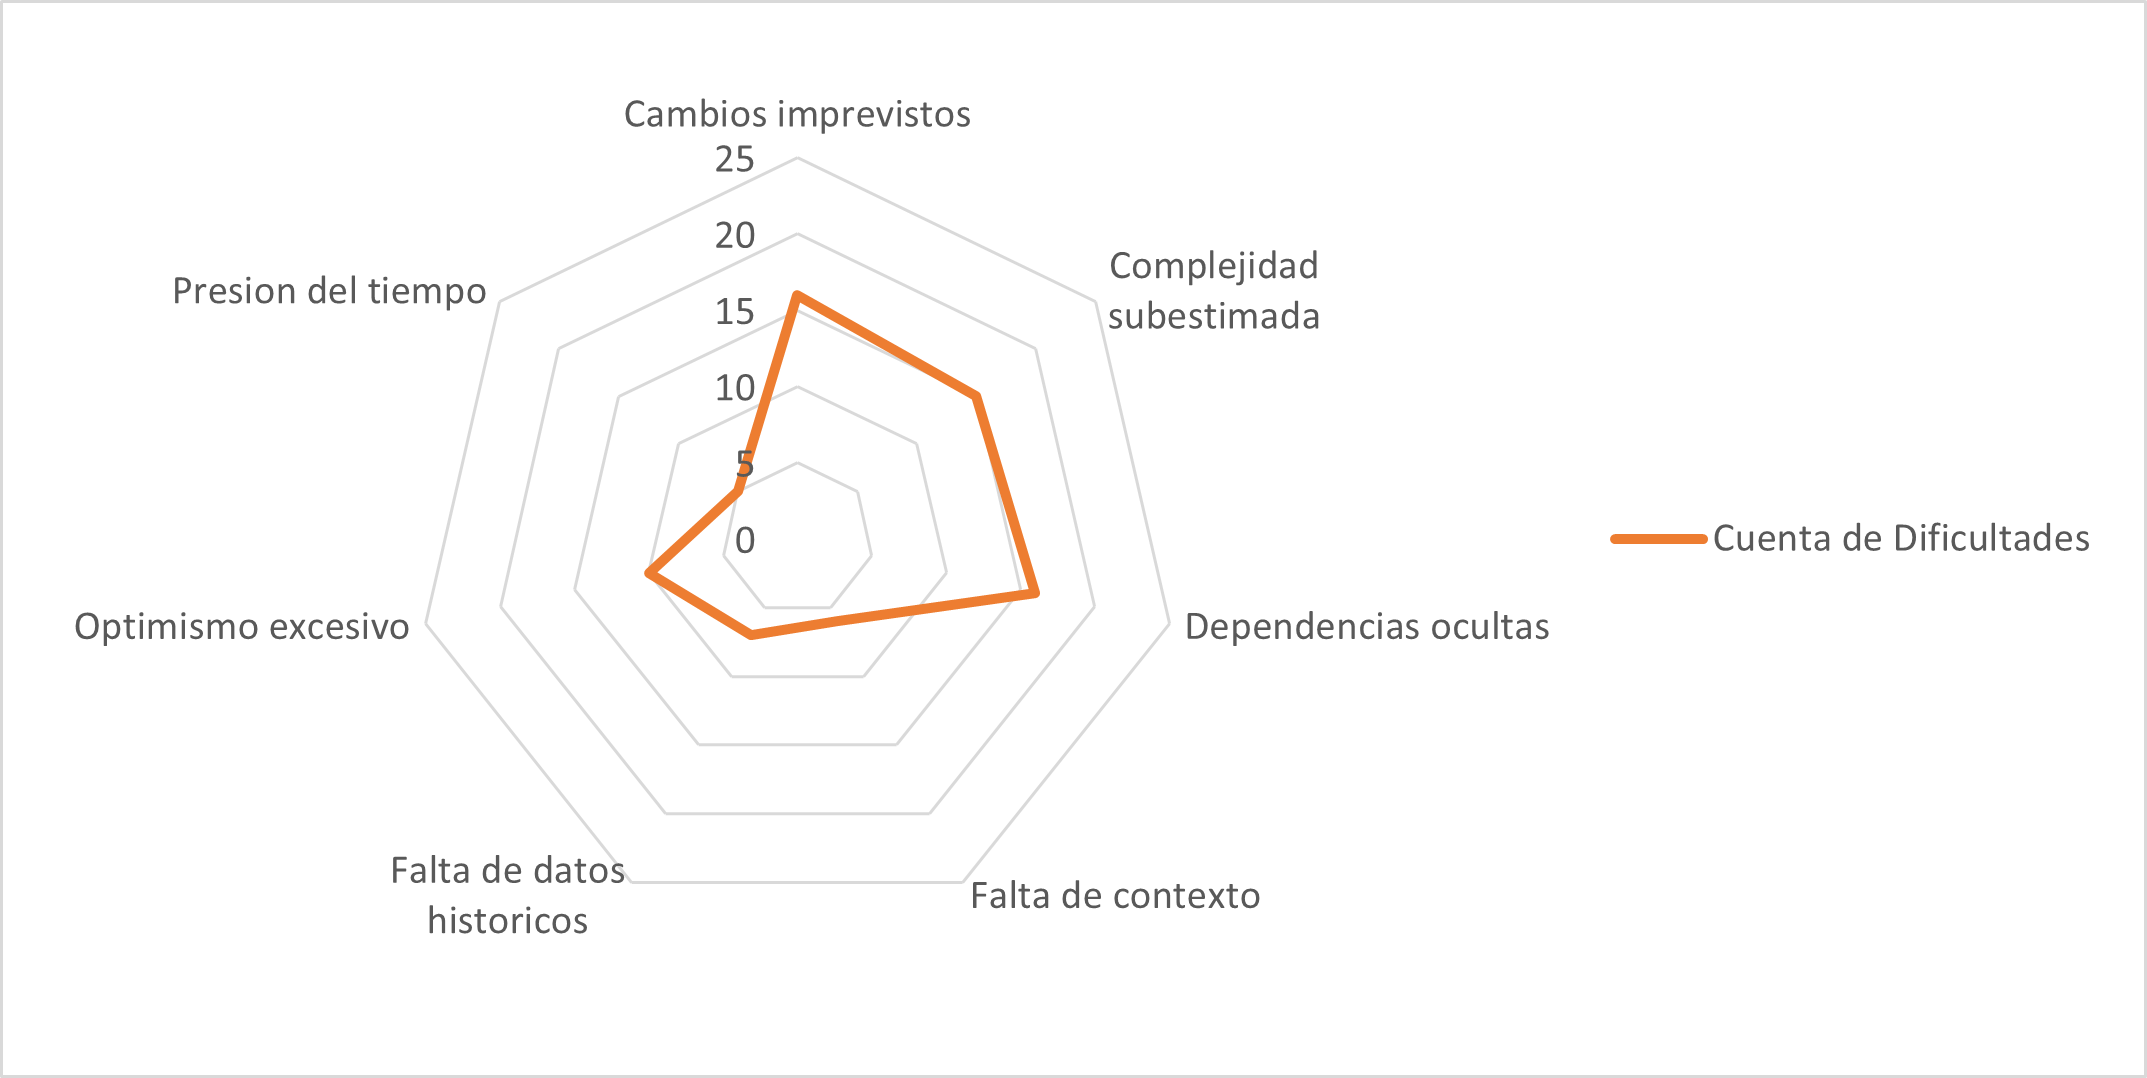
\includegraphics[width=0.45\textwidth]{images/dificultades.png}
    \caption{Utilización de control de versiones en bases de datos por profesión}
    \label{fig:dificultades}
\end{figure}

Por otra parte, cuando se les pregunto a los participantes sobre su experiencia en CI/CD con bases de datos, se observó una adopción limitada. Aunque muchos de los encuestados usan prácticas de CI/CD en desarrollo de software, solo una minoría las aplica específicamente a bases de datos. Los beneficios identificados incluyen la detección temprana de errores y una colaboración mejorada, mientras que los desafíos más citados son la consistencia de datos y la complejidad para integrar cambios de esquema en pipelines automatizados.

Además de las encuestas a profesionales, también se realizó una entrevista con el experto Don Humberto Fonseca Conejo, quien cuenta con una amplia experiencia de más de 15 años en bases de datos, brindando perspectivas profundas sobre los desafíos y prácticas actuales en este campo, lo cual enriquece el análisis de esta investigación. Don Humberto compartió sus opiniones sobre la gestión de cambios en bases de datos, resaltando su preferencia por enfoques tradicionales, como el uso de copias de seguridad y snapshots, en lugar de herramientas de versionado como Liquibase y Flyway. Aunque no está familiarizado con el término "base de datos evolutiva," interpreta este concepto como una base de datos que requiere adaptarse continuamente para cumplir con las demandas cambiantes del negocio.

Al ser consultado sobre la automatización de despliegue de cambios, Don Humberto expresó interés en esta práctica como un método para agilizar procesos y reducir tiempos en entornos multiambiente, aunque destaca que intentos previos no tuvieron éxito debido a la falta de guías y conocimientos técnicos específicos. Sin embargo, reconoce el potencial de herramientas de gestión de versiones en equipos que operan en entornos de alta frecuencia de cambio, afirmando que podrían mejorar el control de versiones y la colaboración en estos escenarios. Estos valiosos aportes subrayan la relevancia de adoptar y adaptar prácticas de versionado y despliegue continuo en el contexto de bases de datos evolutivas, respaldando así los enfoques propuestos en este estudio.


\section{Marco Propuesto}
La propuesta de solución para el control de versiones en bases de datos evolutivas se diseñada para abordar los desafíos en la gestión de cambios en bases de datos, particularmente dentro del contexto de metodologías ágiles y prácticas de CI/CD. La arquitectura planteada permite a los equipos de desarrollo rastrear, revertir y desplegar cambios de manera eficiente y segura, minimizando los riesgos de errores y conflictos en los esquemas de bases de datos, mejorando la colaboración y asegurando la integridad de los datos a lo largo de todo el ciclo de vida del desarrollo.

La metodología propuesta se apoya en herramientas como Liquibase y Flyway, enfocándose en su capacidad para gestionar cambios y automatizar migraciones en bases de datos. A través de un enfoque iterativo e incremental, la arquitectura fue refinada y adaptada a las necesidades específicas del proyecto, resultando en una solución robusta y flexible que puede integrarse en flujos de trabajo ágiles de CI/CD. Esta solución incluye una guía detallada para la implementación de control de versiones en bases de datos, ofreciendo recomendaciones basadas en la evaluación de las herramientas mencionadas y contribuyendo a mejorar los procesos de desarrollo y despliegue en entornos de bases de datos.

A continuacion se describen las dos herramientas antes mencionadas para esta propuesta:
\subsection{Liquibase}
Liquibase es una herramienta de código abierto ampliamente utilizada para el control de versiones en bases de datos. Ofrece funcionalidades clave, como la compatibilidad con bases de datos SQL y NoSQL, la reversión de cambios (rollback) y la integración con herramientas de CI/CD como Jenkins y GitHub Actions. Estas características permiten una gestión eficaz de las modificaciones en el modelo de datos, asegurando la trazabilidad y minimizando el riesgo de errores en los entornos de desarrollo, prueba y producción.\\ Además, Liquibase permite definir cambios en formatos como XML, YAML, JSON o SQL, lo que brinda flexibilidad a los equipos de desarrollo y facilita su integración en proyectos de diferentes escalas.

Para organizar los cambios, Liquibase utiliza un archivo principal denominado \textit{changelog}, que contiene una lista cronológica de cambios estructurada en \textit{changesets} como podemos verlo en la Figura \ref{fig:changelogFig}. Cada \textit{changeset} es una unidad atómica de cambio que incluye un identificador único, el autor y las instrucciones para realizar el cambio, como sentencias SQL o referencias a archivos SQL externos. En este proyecto, se utiliza el formato YAML para el \textit{changelog} por su simplicidad y claridad. A través del \textit{changelog}, Liquibase asegura que los cambios se apliquen de manera ordenada, controlada y consistente, particularmente en entornos de CI/CD, reduciendo el riesgo de conflictos y facilitando la implementación de actualizaciones.

\begin{figure}[H]
    \centering
    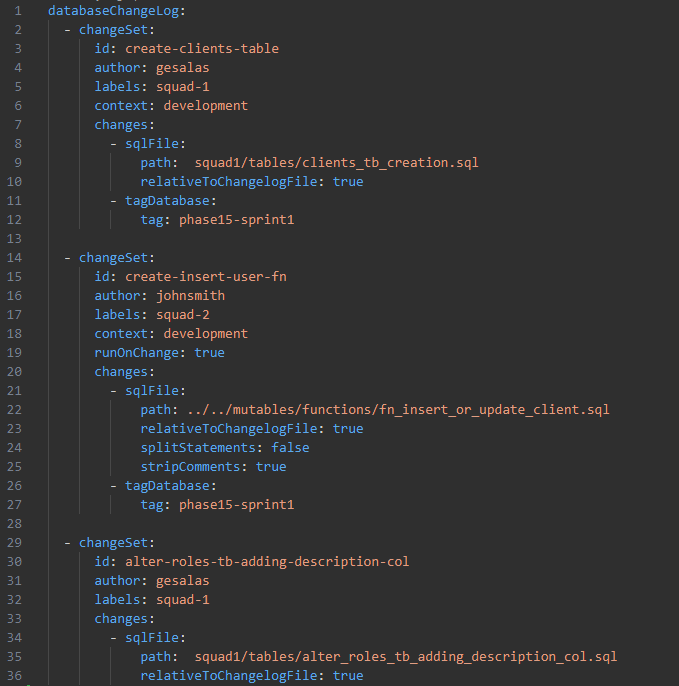
\includegraphics[width=0.48\textwidth]{images/changelogExample.png}
    \caption{Ejemplo de Changelog de Liquibase}
    \label{fig:changelogFig}
\end{figure}

La configuración del proyecto con Liquibase requiere un archivo \texttt{liquibase.properties} que especifica la conexión a la base de datos y el \textit{changelog} principal en el cual se iran agregando los cambios que queramos ejecutar en el proyecto, como e puede ver en la Figura \ref{fig:liquibasePropertiesExample}. Este enfoque también permite que los desarrolladores y DBAs trabajen directamente sobre archivos \texttt{.sql} para realizar modificaciones, aprovechando la trazabilidad de Liquibase. En algunos casos, como en los scripts de datos que necesitan ejecutarse múltiples veces, es posible configurar el \textit{changeset} con la opción \texttt{runOnChange}, lo que permite ejecutar el script cada vez que se despliegue.

\begin{figure}[H]
    \centering
    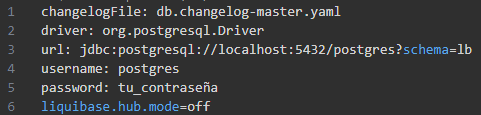
\includegraphics[width=0.48\textwidth]{images/liquibasePropertiesExample.png}
    \caption{Ejemplo del archivo de configuración "liquibase.properties" de Liquibase}
    \label{fig:liquibasePropertiesExample}
\end{figure}

Para la ejecución de los cambios, Liquibase emplea el comando \texttt{liquibase update}, que aplica únicamente los \textit{changesets} aún no registrados en la tabla \textbf{DATABASECHANGELOG}. Esta tabla, creada en la base de datos, mantiene un registro detallado de cada \textit{changeset} ejecutado, incluyendo el ID, autor, fecha y checksum, lo que verifica la integridad de los cambios. Este sistema asegura que los cambios no se dupliquen, y permite que Liquibase mantenga una secuencia controlada, respetando dependencias entre objetos para evitar errores. Así, Liquibase optimiza el control de versiones en bases de datos relacionales, integrándose eficazmente en entornos de desarrollo ágiles y facilitando la gestión de cambios.\\

La organización efectiva de los cambios en la base de datos de un proyecto de control de versiones con Liquibase requiere una jerarquía de carpetas clara y estandarizada, como se ilustra en la Figura \ref{fig:folderHerarchyLiquibase}. Esta estructura permite gestionar de manera ordenada los archivos modificables e inmutables, y facilita la trazabilidad de los cambios al dividir el proyecto en fases, sprints y equipos (squads). A continuación, se presenta la propuesta de jerarquía de carpetas para un proyecto bajo metodología ágil, estructurada en fases y sprints, donde cada fase representa una iteración de desarrollo.

\begin{figure}[H]
    \centering
    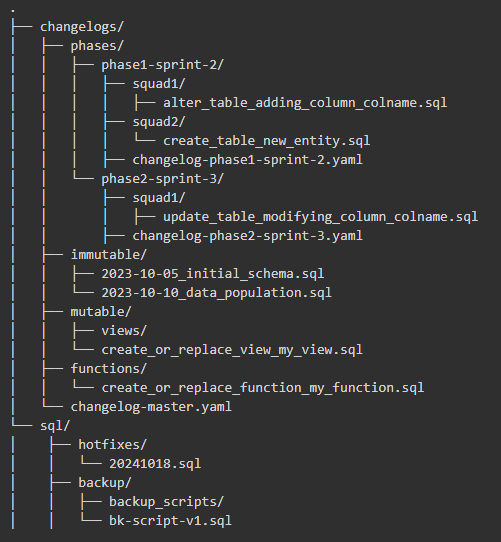
\includegraphics[width=0.48\textwidth]{images/folderHerarchyLiquibase.png}
    \caption{Ejemplo de jerarquía de carpetas propuesta para Liquibase}
    \label{fig:folderHerarchyLiquibase}
\end{figure}

 La siguiente descripción detalla las carpetas principales y su función en el control de versiones utilizando Liquibase:

\begin{itemize}
    \item \textbf{changelogs/}: Carpeta principal para todos los archivos de cambios. Contiene todos los changelogs y los archivos SQL que están directamente relacionados con los cambios aplicados a la base de datos. Es el corazón de la estructura de cambios en tu base de datos.
    
    \item \textbf{phases/}: Dentro de esta carpeta se organizan los cambios en subcarpetas que representan las fases y los sprints del proyecto. El formato utilizado para nombrar cada subcarpeta es \texttt{phaseX-sprint-Y}, donde \texttt{X} representa el número de la fase del proyecto y \texttt{Y} representa el número del sprint.
    
    \item \textbf{squadX/}: Cada fase y sprint tendrá su propio subdirectorio para los cambios realizados por los squads. En estas carpetas se almacenarán los archivos SQL correspondientes a los cambios específicos que realiza cada equipo.
    
    \item \textbf{immutable/}: Carpeta destinada a los archivos no modificables. Aquí se almacenan los cambios iniciales y los scripts que, una vez ejecutados, no deben alterarse. Estos archivos representan una parte crítica de la historia del proyecto y son inmutables para asegurar que el historial de la base de datos se mantenga íntegro.
    
    \item \textbf{mutable/}: Aquí se almacenan los objetos que pueden modificarse y recrearse a lo largo del tiempo, como vistas y funciones. Estos objetos son esenciales para la evolución de la base de datos. Su naturaleza mutable implica que pueden ser recreados en múltiples sprints dependiendo de las necesidades del proyecto. Las vistas se almacenan en el subdirectorio \texttt{mutable/views/}, mientras que las funciones de la base de datos se encuentran en \texttt{mutable/functions/}.
\end{itemize}

Características principales de Liquibase:

\begin{itemize}
    \item \textbf{Compatibilidad con múltiples bases de datos}: Soporta bases de datos SQL y NoSQL, permitiendo su uso en entornos con diferentes sistemas de gestión de bases de datos.
    \item \textbf{Rollback o reversión de cambios}: Permite deshacer cambios aplicados previamente, asegurando una recuperación controlada en caso de errores.
    \item \textbf{Integración con herramientas CI/CD}: Se integra con plataformas como Jenkins y GitHub Actions, facilitando la automatización del despliegue y la sincronización de cambios.
    \item \textbf{Formatos de definición de cambios flexibles}: Ofrece opciones para definir cambios en varios formatos como XML, YAML, JSON o SQL, proporcionando flexibilidad para distintos equipos de desarrollo.
    \item \textbf{Changelog y changesets}: Organiza los cambios en un archivo de \textit{changelog} que estructura los cambios en \textit{changesets} atómicos, los cuales incluyen un identificador único, autor y detalles del cambio.
    \item \textbf{Registro de cambios en la base de datos}: Utiliza la tabla \textbf{DATABASECHANGELOG} para registrar el historial de cambios, garantizando la trazabilidad y la integridad de cada actualización.
    \item \textbf{Comando de actualización controlada}: Ejecuta el comando \texttt{liquibase update} para aplicar solo los cambios nuevos, evitando duplicados y controlando la secuencia de ejecución.
    \item \textbf{Configuración personalizada}: Admite configuraciones específicas en el archivo \texttt{liquibase.properties}, permitiendo conexiones personalizadas.
\end{itemize}

\subsection{Flyway}
Flyway es una herramienta de migración de base de datos que utiliza archivos SQL o código Java para aplicar cambios secuenciales y versionados a la base de datos. A diferencia de Liquibase, que emplea archivos de control llamados changelogs, Flyway sigue una convención de nombres simple para versionar los archivos SQL y asegura que se ejecuten en el orden correcto. Los cambios en la base de datos se aplican a través de archivos de migración, los cuales tienen un formato de nombres específico que permite a Flyway controlar el orden en que se aplican. 

Cada archivo de migración comienza con un prefijo \textit{V} seguido de un número de versión por ejemplo, \texttt{V1\_\_, V2\_\_, etc.}, lo que asegura que los cambios se ejecuten secuencialmente en función del número de versión. Flyway también soporta correcciones a través de archivos especiales que comienzan con \texttt{R\_\_} en lugar de \texttt{V\_\_}, lo que permite aplicar cambios repetidos como en el caso de vistas y funciones.

La configuración de Flyway requiere el archivo llamado \texttt{flyway.conf} Figura \ref{fig:flywayPropertiesExample}, donde se especifican parámetros clave como la conexión a la base de datos, el directorio donde se encuentran los scripts de migración, y otras configuraciones relevantes. Estos parámetros incluyen la URL de la base de datos, las credenciales de acceso, el esquema de destino y la ubicación de los archivos de migración. Además, el parámetro \texttt{flyway.baselineOnMigrate} permite establecer un punto de partida para bases de datos que ya contienen datos, facilitando la integración de Flyway en proyectos existentes.

\begin{figure}[H]
    \centering
    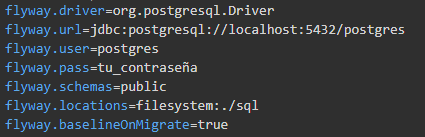
\includegraphics[width=0.48\textwidth]{images/flywayPropertiesExample.png}
    \caption{Ejemplo de archivo de configuración de Flyway}
    \label{fig:flywayPropertiesExample}
\end{figure}

La jerarquía de carpetas en Flyway es sencilla como se muestra en la Figura \ref{fig:folderHerarchyFlyway}, siguiendo una convención en la que los archivos de migración versionados comienzan con \texttt{V\_\_} y los archivos de migración repetibles con \texttt{R\_\_}. Los archivos \texttt{V\_\_} se aplican secuencialmente según el número de versión, mientras que los archivos \texttt{R\_\_} son ejecutados cada vez que se detectan cambios. Esta estructura organizada facilita la gestión de las migraciones y asegura que se apliquen en el orden correcto.

\begin{figure}[H]
    \centering
    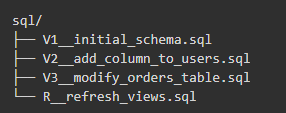
\includegraphics[width=0.48\textwidth]{images/folderHerarchyFlyway.png}
    \caption{Ejemplo de jerarquía de carpetas propuesta para Flyway}
    \label{fig:folderHerarchyFlyway}
\end{figure}

Los archivos SQL son fundamentales en Flyway para gestionar las migraciones. Estos archivos contienen los scripts que Flyway ejecuta secuencialmente para realizar los cambios en la base de datos. La convención de nombres de los archivos garantiza que se sigan las secuencias adecuadas para las migraciones versionadas y repetibles. Cada archivo SQL es ejecutado una sola vez, en el caso de las migraciones versionadas, y repetidamente, en el caso de las migraciones repetibles.

Flyway proporciona una serie de comandos útiles para la gestión de migraciones. El comando \texttt{flyway migrate} se utiliza para aplicar todas las migraciones pendientes, mientras que \texttt{flyway info} permite obtener información sobre el estado de las migraciones aplicadas. Además, el comando \texttt{flyway repair} se utiliza para reparar la tabla de historial en caso de inconsistencias. Los cambios realizados se registran en una tabla llamada \texttt{flyway\_schema\_history}, que mantiene un historial detallado de las migraciones aplicadas, incluyendo el número de versión, la descripción, la fecha de ejecución y el resultado de la migración. Esta tabla es crucial para evitar la duplicación de migraciones y permite el seguimiento de los errores en el proceso de migración. \\

Las principales características de Flyway son las siguientes:

\begin{itemize}
    \item \textbf{Convención de nombres para archivos de migración}: Los archivos de migración versionados comienzan con \texttt{V\_\_} seguido de un número de versión (ej. \texttt{V1\_\_}), mientras que los archivos de migración repetibles comienzan con \texttt{R\_\_}.
    \item \textbf{Ejecución secuencial de migraciones}: Los archivos de migración son ejecutados en orden según su número de versión.
    \item \textbf{Soporte para correcciones}: Los archivos de corrección (\texttt{R\_\_}) se ejecutan repetidamente, lo cual es útil para cambios frecuentes como en vistas y funciones.
    \item \textbf{Registro de historial de migraciones}: Flyway mantiene una tabla llamada \texttt{flyway\_schema\_history} donde guarda información sobre todas las migraciones aplicadas, incluyendo la versión, descripción, fecha de ejecución y resultado.
    \item \textbf{Configuración mediante flyway.conf}: En el archivo de configuración \texttt{flyway.conf} se especifican parámetros clave como la URL de la base de datos, las credenciales de acceso, el esquema de destino y la ubicación de los archivos de migración.
    \item \textbf{Migraciones aplicadas automáticamente}: Flyway aplica todas las migraciones pendientes al ejecutar el comando "\texttt{flyway migrate}".
    \item \textbf{Soporte para bases de datos existentes}: Flyway permite establecer un punto de partida para bases de datos que ya contienen datos mediante el parámetro "\texttt{flyway.baselineOnMigrate}".
    \item \textbf{Integración con CI/CD}: Flyway se puede integrar fácilmente en pipelines de CI/CD para automatizar el proceso de migración de bases de datos.
\end{itemize}


\subsection{GitOps para bases de datos relacionales}
En el caso de bases de datos, aplicar GitOps significa gestionar los cambios de esquema y migraciones a través de pipelines de CI/CD, asegurando que los despliegues de la base de datos sean consistentes, seguros y completamente automatizados. Este enfoque permite que las migraciones de bases de datos sean tratadas como código, lo que mejora la trazabilidad, la consistencia y la eficiencia en los despliegues.GitOps es un enfoque que automatiza la gestión de infraestructura y aplicaciones mediante la sincronización de estados declarativos almacenados en un repositorio Git con los entornos de producción.\\ 
El flujo GitOps propuesto para la base de datos sigue los siguientes pasos:

\begin{itemize}
    \item \textbf{Control de cambios con Git:} Todas las migraciones de la base de datos se almacenan en un repositorio Git. Los archivos de migración de Liquibase o Flyway (changelogs, scripts SQL) se versionan y son revisados mediante pull requests.
    \item \textbf{Integración Continua (CI):} Cada vez que se sube un cambio (una nueva migración de base de datos) al repositorio Git, un pipeline CI valida la integridad del código SQL. Un SQL linter como SQLFluff puede ser utilizado en este proceso para verificar que los scripts sigan las mejores prácticas de estilo y calidad. Además, se ejecutan pruebas automáticas en un entorno de base de datos de prueba para verificar que las migraciones no rompan la integridad del esquema.
    \item \textbf{Despliegue Continuo (CD):} Si las pruebas CI son exitosas, el pipeline de CD es activado y los cambios de la base de datos se despliegan de forma automatizada en entornos como staging y producción. Dependiendo de la herramienta utilizada (Liquibase o Flyway), se ejecutarán las migraciones correspondientes para garantizar que la base de datos esté sincronizada con el estado actual del código en el repositorio Git.
\end{itemize}

\subsection{SQL Linter}
Un SQL linter es una herramienta diseñada para analizar el código SQL y detectar posibles errores, inconsistencias o malas prácticas antes de que se ejecuten en la base de datos. Al igual que los linters utilizados en otros lenguajes de programación, un linter de SQL ayuda a mejorar la calidad del código, asegurando que se adhiera a los estándares de codificación establecidos y que sea fácil de mantener y entender. El uso de un linter en los proyectos de bases de datos es crucial, ya que garantiza que el código SQL esté optimizado, siga convenciones predefinidas, y evite errores comunes como errores de sintaxis, inconsistencias y malas prácticas.

En esta solución se propone utilizar \texttt{SQLFluff}, un linter extensible y configurable para SQL, ideal para proyectos que involucren diversas plataformas de bases de datos como PostgreSQL, MySQL y SQL Server. \texttt{SQLFluff} es una herramienta de código abierto que soporta múltiples dialectos SQL, lo que lo convierte en una opción versátil para entornos con diferentes bases de datos. Su integración en los procesos de desarrollo e implementación asegura que las consultas SQL sigan las mejores prácticas antes de ser enviadas a producción, lo que ayuda a mantener la calidad del código en todo momento. Además, \texttt{SQLFluff} es altamente adaptable, permitiendo la creación de reglas personalizadas que se ajustan a los estándares de codificación específicos de cada equipo o proyecto. Su capacidad para integrarse en pipelines de CI/CD facilita la verificación del código SQL antes del despliegue, garantizando el cumplimiento de las convenciones establecidas. También puede analizar archivos \texttt{.sql}, detectando errores como inconsistencias en mayúsculas, problemas de formato o uso incorrecto de columnas, y ofrece autocorrección para adoptar un estilo uniforme en los proyectos de manera más eficiente.

\subsection{Configuración de SQLFluff}
El primer paso para incorporar \texttt{SQLFluff} es su instalación. Dado que se basa en Python, es recomendable contar con un entorno de desarrollo en Python bien configurado. Una vez asegurado esto, se puede instalar \texttt{SQLFluff} utilizando el gestor de paquetes de Python "\texttt{pip}", mediante el comando \texttt{pip install sqlfluff}. Esto facilita su integración en cualquier flujo de trabajo automatizado. Es importante aclarar que Python no es obligatorio para el uso de \texttt{SQLFluff}, pero es la opción más directa y sencilla.

Para que \texttt{SQLFluff} se comporte de acuerdo con las reglas del proyecto, es necesario un archivo de configuración específico, el cual debe ser llamado \texttt{.sqlfluff} y debe de estar en la raíz del proyecto. Este archivo define aspectos clave como el dialecto de base de datos, la longitud máxima de líneas, el estilo de indentación, entre otros. En la Figura \ref{fig:sqlFluffConfigExample}, se muestra un ejemplo de la configuración de SQLFluff para un proyecto que usa PostgreSQL como base de datos:

\begin{figure}[H]
    \centering
    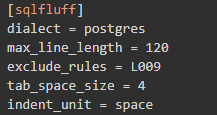
\includegraphics[width=0.42\textwidth]{images/sqlFluffConfigExample.png}
    \caption{Ejemplo de archivo de configuración para sqlfluff}
    \label{fig:sqlFluffConfigExample}
\end{figure}


\subsection{Configuración de Pre-Commit}
Para asegurar que ningún script SQL llegue al repositorio con errores de estilo o formato, podemos integrar \texttt{SQLFluff} con \texttt{pre-commit}, de manera que cada vez que un desarrollador intente hacer un commit, el código SQL sea analizado automáticamente. Esto añade una capa adicional de control, asegurando que el código SQL que se integra cumpla con las reglas del proyecto. Para integrar \texttt{pre-commit}, debemos instalarlo utilizando el manejador de paquetes de Python, \texttt{pip}, mediante el comando \texttt{pip install pre-commit}. Luego, se configura un archivo llamado \texttt{.pre-commit-config.yaml}, Figura \ref{fig:precommitExample} que define los hooks que \texttt{SQLFluff} ejecutará antes de cada commit que se quiera agregar al repositorio.

Esto permite que cada vez que se haga un commit, \texttt{SQLFluff} valide los archivos \texttt{.sql} y si es posible, corrija automáticamente algunos errores de estilo sin intervención manual. Además, cabe aclarar que \texttt{SQLFluff} puede ejecutarse manualmente sobre los scripts SQL del proyecto utilizando la terminal del sistema. Esto es útil cuando se quiere revisar el código de manera proactiva antes de hacer cualquier cambio significativo. En este caso, el comando para ejecutar la revisión del código sería \texttt{sqlfluff lint <nombre\_del\_archivo.sql>}, y en caso de querer corregir los errores encontrados, se ejecutaría \texttt{sqlfluff fix <nombre\_del\_archivo.sql>}. Si se desea ejecutar la revisión sobre todo el proyecto, solo basta con reemplazar el nombre del archivo por un punto, un ejemplo de esto sería: "\texttt{sqlfluff fix .}".

\begin{figure}[H]
    \centering
    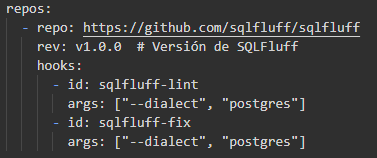
\includegraphics[width=0.48\textwidth]{images/precommitExample.png}
    \caption{Ejemplo de archivo de configuración para pre-commit en proyecto con sqlfluff}
    \label{fig:precommitExample}
\end{figure}


\subsection{Consideraciones de la implementación}
Ambas herramientas, Liquibase y Flyway, se integran perfectamente en un entorno GitOps con PostgreSQL, proporcionando trazabilidad completa de los cambios en la base de datos. Al utilizar un repositorio Git como la fuente de verdad y un linter para SQL que nos ayude a mantener algunas reglas entre los miembros del equipo de desarrollo, se asegura que cualquier modificación en la base de datos esté bien documentada y pueda ser revisada, probada y desplegada de forma controlada. Además, tanto Liquibase como Flyway mantienen una tabla interna (\texttt{databasechangelog} en Liquibase y \texttt{flyway\_schema\_history} en Flyway) en la base de datos para registrar las migraciones aplicadas. Estas tablas son esenciales para el correcto funcionamiento de los despliegues automatizados, y es importante considerar las capacidades de rollback que ofrecen las herramientas, siendo más flexible en Liquibase que en Flyway, ya que este último depende más de scripts SQL orientados a versiones.


\section{Conclusiones y Trabajos Futuros}
Este proyecto ha explorado la implementación de un sistema de control de versiones en bases de datos altamente cambiantes, proponiendo herramientas como Liquibase y Flyway en el contexto de metodologías ágiles y prácticas de CI/CD. A continuación, se presentan las conclusiones obtenidas y algunas recomendaciones para futuras investigaciones.

\subsection{Conclusiones}
El análisis realizado en este proyecto destaca la importancia de implementar un control de versiones efectivo en bases de datos, especialmente en entornos que utilizan metodologías ágiles y prácticas de CI/CD. Una de las principales conclusiones es que la falta de un sistema y/o proceso de control de versiones bien definido puede llevar a problemas significativos, como el seguimiento de los cambios aplicados, dificultades en la gestión de dependencias y conflictos en la colaboración entre los miembros del equipo de desarrollo. 

La comparación entre Liquibase y Flyway ha demostrado que ambas herramientas ofrecen capacidades sólidas para gestionar cambios en las bases de datos, aunque cada una tiene sus ventajas específicas. Liquibase, por ejemplo, es particularmente fuerte en su soporte para múltiples bases de datos y su flexibilidad en la gestión de cambios complejos. Por otro lado, Flyway destaca por su simplicidad y facilidad de uso, lo que lo convierte en una opción atractiva para proyectos donde la curva de aprendizaje debe ser mínima. En general, al comparar el resultado de las encuestas y la entrevista se puede concluir que la adopción de cualquiera de estas herramientas, en combinación con prácticas ágiles y CI/CD, puede mejorar de diferentes maneras la eficiencia y la calidad con la que se implementan cambios en los esquemas de bases de datos.


\subsection{Trabajos Futuros}
A partir de los hallazgos de este proyecto, se recomienda que las organizaciones que aún no han adoptado un sistema de control de versiones en sus bases de datos consideren la implementación de herramientas como Liquibase o Flyway. Es crucial seleccionar la herramienta que mejor se adapte a las necesidades específicas del proyecto y del equipo de desarrollo, considerando factores como la complejidad de los cambios en la base de datos, la diversidad de los sistemas de bases de datos utilizados y el nivel de experiencia del equipo. 

Además, se recomienda que estas herramientas se integren dentro de un marco de trabajo ágil y de CI/CD, para maximizar los beneficios en términos de automatización y colaboración. Las organizaciones deben también considerar la capacitación de sus equipos en el uso de estas herramientas y en la estimación de esfuerzos para los cambios en bases de datos, lo que puede incluir la adopción de prácticas como la planificación basada en puntos de historia. 
Por último, es esencial que se realicen pruebas continuas y ajustes en la implementación para asegurar que el sistema de control de versiones esté alineado con las necesidades cambiantes del proyecto y que se minimicen los riesgos de problemas de integridad y consistencia de datos en el entorno de producción.



\renewcommand{\refname}{Referencias}
\nocite{}
\bibliography{references}
\bibliographystyle{IEEEtran}

    
\end{document}

